\documentclass[twocolumn]{article}
\usepackage[spanish]{babel}
\usepackage[utf8]{inputenc}
\usepackage{amssymb}
\usepackage{graphicx}
\usepackage{verbatim}
\usepackage{algorithmic}
\usepackage{enumitem}
\setlist{nolistsep}




\author{
Nombre:....................................... \\
    Departamento de Informática y Sistemas \\
    Universidad EAFIT \\
}
\title{
    Estructuras de Datos 2 - ST0247 - 032 \\
    Examen Parcial 1 (jueves)
}
\date{
    Marzo 23, 2017
}

\begin{document}
\vspace{-5cm}
\maketitle


\section*{Criterios de calificación}

\begin{itemize}
\item Selección múltiple con única respuesta
\begin{itemize}
\item Respuesta correcta: 100\%
\item Respuesta incorrecta: 0\%
\end{itemize}

\item Completar código
\begin{itemize}
\item Respuesta correcta 100\%
\item Respuesta incorrecta o vacía 0\%
\end{itemize}
\end{itemize}

\vspace{1cm}

\textbf{NOTAS IMPORTANTES:}
\begin{itemize}
	\item Responda en la hoja de PREGUNTAS
	\item Marque la hoja de PREGUNTAS
\end{itemize}


\section{Implementación grafos 20\%}
Considere el siguiente grafo:

\begin{center}
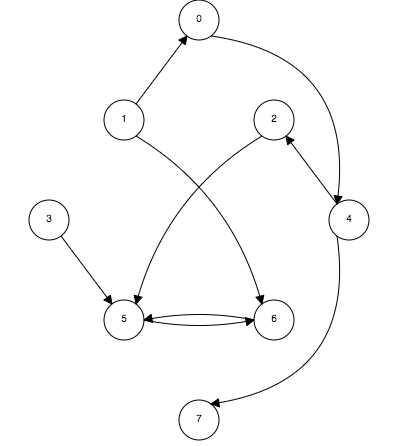
\includegraphics[scale=0.5]{grafin2.png}
\end{center}

\begin{enumerate}[label=\Alph*]
	\item (10\%) Complete la representación de \textbf{matrices de adyacencia}. Si no hay arco,
  por simplicidad, deje el espacio en blanco.

\begin{center}
\begin{tabular}{| c | c | c | c | c | c | c | c | c |}
\hline
  & 0 & 1 & 2 & 3 & 4 & 5 & 6 & 7 \\
\hline
0 &   &   &   &   & 1  &   &   &   \\
\hline
1 &  1 &   &   &   &   &   &  1 &   \\
\hline
2 &   &   &   &   &   &   &   &   \\
\hline
3 &   &   &   &   &   &   &   &   \\
\hline
4 &   &   &   &   &   &   &   &   \\
\hline
5 &   &   &   &   &   &   &   &   \\
\hline
6 &   &   &   &   &   &   &   &   \\
\hline
7 &   &   &   &   &   &   &   &   \\ 
\hline
\end{tabular}
\end{center}

	\item (10\%) Complete la representación de \textbf{listas de adyacencia}. Como
  el grafo no tiene pesos, sólo se colocan los sucesores en la lista de adyacencia.\\


$0 \rightarrow (4,1)$\\
$1 \rightarrow$\\
$2 \rightarrow$\\
$3 \rightarrow$\\
$4 \rightarrow$\\
$5 \rightarrow$\\
$6 \rightarrow$\\
$7 \rightarrow$\\


\end{enumerate}



\section{Recorridos de grafos 20\%}

Para el grafo anterior, complete la salida
que darían los siguientes algoritmos:


\begin{enumerate}[label=\Alph*]
	\item (10\%) Complete el orden en que se recorren los nodos usando \textbf{búsqueda en profundidad} (en Inglés DFS) a partir de cada nodo. Si hay varias opciones de recorrer el grafo con DFS, elija siempre el vértice más pequeño.\\


$0 \rightarrow 4 \rightarrow 2 \rightarrow 5 \rightarrow 6 \rightarrow 7 $\\
$1 \rightarrow$\\
$2 \rightarrow$\\
$3 \rightarrow$\\
$4 \rightarrow$\\
$5 \rightarrow$\\
$6 \rightarrow$\\
$7 \rightarrow$\\


\item (10\%) Complete el orden en que se recorren los nodos usando \textbf{búsqueda en amplitud} (en Inglés BFS) a partir de cada nodo. Si hay varias opciones de recorrer el grafo con BFS, elija siempre el vértice más pequeño.\\


$0 \rightarrow 4 \rightarrow 2 \rightarrow 7 \rightarrow 5 \rightarrow 6 $\\
$1 \rightarrow$\\
$2 \rightarrow$\\
$3 \rightarrow$\\
$4 \rightarrow$\\
$5 \rightarrow$\\
$6 \rightarrow$\\
$7 \rightarrow$\\


\end{enumerate}

\section{Fuerza bruta 20\%}

La función \texttt{ordenar} es un algoritmo de ordenamiento, de menor a mayor, por fuerza bruta. Dicho algoritmo calcula todas
las permutaciones posibles de un arreglo \texttt{arr} hasta
encontrar una permutación donde los elementos están ordenados (es decir, cuando \texttt{estaOrdenado} retorna verdadero).
Tenga en cuenta que \texttt{ordenar} imprime en la pantalla el arreglo \texttt{arr} ordenado, pero no necesariamente deja el arreglo
\texttt{a} ordenado por la forma en que está diseñado el algoritmo. Aunque esto último no es deseable, ese no es el problema de este parcial.

{\small
\begin{verbatim}
static boolean estaOrdenado(int[] a) {
       for (int i = 0; i < a.length - 1; i++)
           if (a[i] > a[i + 1]) 
               return false;
       return true;
   }
static void cambiar(int[] arr, int i, int k){
       int t = arr[i];
       arr[i] = arr[k];
       arr[k] = t;
   }
static void ordenar(int[] arr, int k){
        for(int i = k; i < arr.length; i++){
            cambiar(arr, i, k);
            if (estaOrdenado(arr))
                System.out.println(
                    Arrays.toString(arr));  
            ordenar(______, ______);
            cambiar(arr, k, i);
        }
    }
\end{verbatim}
}

\begin{enumerate}[label=\Alph*]
  \item (10\%) Complete los espacios vacíos en el llamado recursivo del método \texttt{ordenar}\\

  \_\_\_\_\_\_\_\_\_\_\_\_, \_\_\_\_\_\_\_\_\_\_\_\_

%ordenar(arr, k+1);

\item (10 \%) Complete la complejidad, en el peor de los casos,
del método \texttt{ordenar}\\

  O(\_\_\_\_)

%O(n!)
\end{enumerate}






\section{Backtracking 30\%}


Wilkenson y Sofronio están aquí de nuevo. En esta vez han traído un juego muy interesante, en el cual Sofronio, en primer lugar, escoge un numero $n$ $(1 \leq n \leq 20)$ y, en segundo lugar, escoge tres números $a, b$ y $c$ $(1 \leq a \leq 9, 1 \leq b \leq 9, 1 \leq c \leq 9)$. Después, Sofronio le entrega estos números a Wilkenson y Wilkenson le tiene que decir a Sofronio \textbf{la cantidad máxima de números, usando  $a$, $b$ y $c$ (se puede tomar un número más de una vez),  que al sumarlos den el valor $n$}. 

Como un ejemplo, si Sofronio escoge $n = 14$ y $a = 3, b = 2, c = 7$. ¿Qué posibilidades hay de sumar 14 con $a, b$ y $c$?\\

\begin{tabular}{l l}
$7 + 7 = 14$  &                  cantidad es 2 \\
$7 + 3 + 2 + 2 = 14$ &          cantidad es 4 \\
$3 + 3 + 3 + 3 + 2 = 14$  &  cantidad es 5 \\
$\dots$ & \\
$2 + 2 + 2 + 2 + 2 + 2 + 2 = 14$ & cantidad es 7 \\\\
\end{tabular}

La cantidad máxima de números es 7. Esta sería la respuesta que da Wilkenson a Sofronio. 
Como Wilkenson es muy astuto, ha diseñado un algoritmo para determinar la cantidad máxima de números y quiere que le ayudes a terminar su código. Asuma que hay al menos una forma de sumar $n$ usando los números $a$, $b$ y $c$ en diferentes cantidades, incluso
si algunos de los números se suman $0$ veces como sucede en el ejemplo anterior.

{\small
\begin{verbatim}
1 int solucionar (int n, int a, int b, int c) 
2   if (n == 0 )
3      return 0;
4   int res = solucionar(____________) + 1;
5   res = Math.max(_______,__________);  
6   res = Math.max(_______,__________);
7   return res;
\end{verbatim}
}

\begin{enumerate}[label=\Alph*]


	\item (10 \%) Complete el espacio de la línea 04\\

	\_\_\_\_\_\_\_\_\_\_\_\_\_\_\_\_\_\_\_\_\_\_\_\_

	\item (10 \%) Complete los espacios de la línea 05\\

	\_\_\_\_\_\_\_\_\_\_\_\_, \_\_\_\_\_\_\_\_\_\_\_\_

	\item (10 \%) Complete los espacios de la línea 06	\\

	\_\_\_\_\_\_\_\_\_\_\_\_, \_\_\_\_\_\_\_\_\_\_\_\_
\end{enumerate} 


% public int solucionar(int n, int a, int b, int c){
% 	//Claramente si n es menor que los otros valores, no se puede obtener ninguna
% 	//combinacion.
% 	if(n == 0 || (n < a && n < b && n < c)){
% 		return 0;
% 	}
% 	//Probemos restando el valor de "a" a n.
% 	int res = solucionar(n - a, a, b, c) + 1;
% 	//Maximicemos el resultado quitandole b a n.
% 	res = max(res, solucionar(n - b, a, b, c) + 1);
% 	//Maximicemos el resultado quitandole c a n.
% 	res = max(res, solucionar(n -c, a, b, c) + 1);	
% 	return res;
% }


\section{Alg. Voraces 10\%}
El problema del \textbf{agente viajero} consiste en responder la siguiente pregunta: Dada
una lista de ciudades y las distancias entre cada par de ciudades, ¿cuál es la
ruta posible más corta que visita a cada ciudad exactamente una vez y regresa a la
ciudad de origen? 

Un algoritmo voraz para solucionar este problem es el \textbf{algoritmo del vecino más
cercano}. El algoritmo empieza en la primera ciudad y selecciona en
cada iteración una nueva ciudad, no visitada, que sea la más cercana a la inmediamente
anterior. A continuación una implementación del algoritmo del vecino más cercano
que recibe como parámetro un grafo representado como matriz de adyacencia. 

La persona que hizo este código es un ingeniero matemático. En Matlab los índices
empiezan en $1$. Por esta razón, el camino que encuentra el algoritmo empieza con la ciudad numerada con $1$ y trabaja
con ciclos \texttt{while} en lugar de \texttt{for}. Adicionalmente, el programador inicia los índices en $1$, por ejemplo \texttt{i = 1}. Por si fuera poco, 
la variable \texttt{min} no era necesaria inicializarla fuera del bloque \texttt{while} y \texttt{minFlag} hubiera sido
mejor declararla dentro del bloque \texttt{while}. Finalmente,
 el arreglo de visitados sería más eficiente haberlo hecho con tipo \texttt{boolean}. No obstante,
 el programa funciona en Java y tiene una complejidad de $O(n^2)$, que es la esperada para este algoritmo.

\begin{verbatim}
01 public void tsp(int adjacencyMatrix[][]) {
02  Stack<Integer> stack = new Stack<Integer>();
03  int numberOfNodes = adjacencyMatrix[1].length - 1;
04  int[] visited = new int[numberOfNodes + 1];
05  visited[1] = 1;
06  stack.push(1);
07  int element, dst = 0, i;
08  int min = Integer.MAX_VALUE;
09  boolean minFlag = false;
10  System.out.print(1 + "\t");
11  while (!stack.isEmpty()) {
12   element = stack.peek();
13   i = 1;
14   min = Integer.MAX_VALUE;
15   while (i <= numberOfNodes) {
16    if (adjacencyMatrix[element][i] > 0 
17        && visited[i] == 0) {
18         if (_______> ______) {
19          min = adjacencyMatrix[element][i];
20          dst = i;
21          minFlag = true;
22         }
23    }
24    i++;
25   }
26   if (minFlag) {
27    visited[dst] = 1;
28    stack.push(dst);
29    System.out.print(dst + "\t");
30    minFlag = false;
31    continue;
32   }
33   stack.pop();
34  }
}
\end{verbatim}

\texttt{Continue} es una palabra reservada en Java que permite terminar una iteración
de un ciclo abruptamente y pasar a la siguiente iteración del ciclo.\\

\begin{enumerate}[label=\Alph*]


    \item (10\%) Complete el espacio en la línea 18\\


  \_\_\_\_\_\_ $>$ \_\_\_\_\_\_

\end{enumerate}

%if (min > adjacencyMatrix[element][i])                       {

\end{document}
